\chapter{Controleren op kwaliteitsgebreken}\label{sec:kwaliteitsgebrek}
In dit hoofdstuk beschrijven we een alternatieve voorstellingsmethode voor klassediagrammen waarmee we bepaalde soorten kwaliteitsgebreken kunnen detecteren. Waar in hoofdstuk \ref{sec:consistentie} objecten centraal stonden, doen we daar hier afstand van: We abstraheren de logische types voor klasses weg en concentreren ons in de plaats op \textit{ClassObject}, een logisch type dat een overeenkomstig object heeft voor alle klasses in het diagram. We gebruiken het diagram in figuur \ref{fig:diagram-voorbeeld} weer als begeleidend voorbeeld. In de volgende subsecties overlopen we hoe we de theorie die we gebruiken voor dit probleem opbouwen.

\section{Gebruikte logische types en predicaten}
\sloppy Waar we in sectie \ref{sec:hierarchies} het logisch type \textit{ClassObject} en het predicaat \textit{IsSupertypeOf/2} afwezen, behouden we deze hier.

We gebruiken daar bijkomend de volgende nieuwe logische symbolen:

\begin{itemize}
	\item \textbf{\textit{BiAssoc(ClassObject,ClassObject)}}: drukt uit dat er een binaire associatie bestaat tussen de twee klasses.
	\item \sloppy \textbf{\textit{BiAssocLow(ClassObject,ClassObject,ClassObject) : nat}}: voor \\ \textit{BiAssocLow(x,y,x) = n1} geldt dat voor de binaire associatie tussen klasse \textit{x} en klasse \textit{y} de ondergrens voor de multipliciteit aan de \textit{x}-kant gelijk is aan \textit{n1}; een gelijkaardige interpretatie geldt voor \textit{BiAssocLow(x,y,y) = n2}.
	\item \textbf{\textit{BiAssocHigh(ClassObject,ClassObject,ClassObject) : nat}}: gelijkaardig aan \textit{BiAssocLow/3}, maar dan voor de bovengrens van de multipliciteit.
\end{itemize}

Verder defini\"eren we een hulppredicaat \textit{EqualNbInstances(ClassObject, ClassObject)} dat uitdrukt dat twee klasses even veel instanties moeten bevatten. De volgende inductieve definitie vult de interpretatie ervan in:

\begin{align*}
	\{
	&\forall{x}[ClassObject]\forall{y}[ClassObject](EqualNbInstances(x, y) \leftarrow BiAssoc(x, y) \\ &\land BiAssocLow(x, y, x) = BiAssocLow(x, y, y) = BiAssocHigh(x, y, x) \\ &= BiAssocHigh(x, y, y)). \\
	&\forall{x}[ClassObject]\forall{y}[ClassObject](EqualNbInstances(x, y) \leftarrow \\ &\exists{z}[ClassObject](EqualNbInstances(x, z) \land EqualNbInstances(z, y))).
	\}
\end{align*}

Het basisgeval stelt dat twee klasses even veel instanties bevatten als ze aan elkaar gerelateerd zijn in een associatie en als de grenzen op beide uiteindes dezelfde zijn. De transitieve sluiting over de bekomen paren vult dan de interpretatie van \textit{EqualNbInstances/2} in.

\section{Kwaliteitsgebreken detecteren}
Er zijn drie kwaliteitsgebreken waarnaar wordt gezocht in de resulterende theorie:

\begin{itemize}
	\item \textbf{\textit{Many-to-many} associaties}: Dit zijn associaties waar de bovengrens van de multipliciteiten aan beide kanten gelijk is aan $*$. Het voorkomen van een \textit{many-to-many} associatie is doorgaans een teken dat er een klasse ontbreekt in het ontwerp. Het is dus van groot belang dat dit wordt opgespoord en opgelost.
	
	\item \textbf{Losstaande klasse}: Concreet is een losstaande klasse een klasse die geen associatie heeft met een andere klasse in het ontwerp. Zulk een klasse is nutteloos en moet ofwel verbonden worden met een andere klasse of verwijderd worden.
	
	\item \textbf{Onvoldoende precieze bovengrens ten gevolge van gelijk aantal instanties}\cite{Balaban2015}: Beschouw figuur \ref{fig:cycle}. De associaties \textit{Alice}---\textit{Bob} en \textit{Bob}---\textit{Charlie} hebben als gevolg dat de klasses \textit{Alice}, \textit{Bob} en \textit{Charlie} even veel instanties hebben. Dit heeft echter tot effect dat in de associatie \textit{Charlie}---\textit{Alice} een instantie van \textit{Charlie} nooit gerelateerd zal zijn tot twee instanties van \textit{Alice}. Dit maakt de bovengrens van 2 op het uiteinde \textit{Alice} dus onvoldoende precies. Aangezien dit effect niet onmiddelijk duidelijk is, lost de ontwerper dit best op om de verstaanbaarheid van het diagram te verbeteren. Als hij wil toelaten dat een instantie van \textit{Charlie} toch gerelateerd kan zijn aan twee instanties van \textit{Alice}, kan hij de ondergrens op het uiteinde \textit{Alice} of de bovengrens op het uiteinde \textit{Charlie} veranderen. De ontwerper heeft de optie om de multipliciteit op \textit{Alice} te veranderen naar $1$ als hij het toch niet nodig vindt dat een instantie van \textit{Charlie} gerelateerd kan zijn aan meerdere instanties van \textit{Alice}. Figuur \ref{fig:cyclegen} toont het algemeen patroon voor dit gebrek voor drie klasses. De associaties \textit{Y}---\textit{Z} en \textit{Z}---\textit{X} dwingen af dat alle drie klasses even veel instanties bevatten. In de associatie \textit{X}---\textit{Y} zorgen de multipliciteit van $k$ op het uiteinde \textit{X} en de ondergrens van $k$ op het uiteinde \textit{Y} ervoor dat een instantie van \textit{X} nooit gerelateerd kan zijn aan meer dan $k$ instanties van \textit{Y}. Analoog aan het geval in figuur \ref{fig:cycle} moet de ontwerper de multipliciteit op \textit{Y} veranderen naar $k$. Als hij toch wil toelaten dat een instantie van \textit{X} gerelateerd kan zijn aan meer dan $k$ instanties van \textit{Y}, verandert hij de ondergrens op het uiteinde \textit{Y} naar $j < k$, of hij verandert de bovengrens op het uiteinde \textit{X} naar $m > k$. Het patroon in figuur \ref{fig:cyclegen} is makkelijk te veralgemenen tot meer dan drie klasses.
\end{itemize}

We defini\"eren deze respectievelijke gebreken in de logische theorie door middel van de volgende logische zinnen:

\begin{align}
	\nonumber \forall{x}[ClassObject]\forall{y}[ClassObject](ManyToMany(x,y) \Leftrightarrow BiAssoc(x,y) \land \\ \lnot\exists{z}[nat](BiAssocHigh(x,y,x) = z) \land \lnot\exists{z}[nat](BiAssocHigh(x,y,y) = z)).\label{form:manytomany}
\end{align}

\begin{align}
	\nonumber \forall{x}[ClassObject](LooseClass(x) \Leftrightarrow \lnot(\exists{y}[ClassObject](\lnot(x = y) \land (BiAssoc(x,y) \\ \lor \exists{s}[ClassObject]\exists{y}[ClassObject](\mathit{IsSupertypeOf}(s,x) \land BiAssoc(s,y)))))).\label{form:loose}
\end{align}

\begin{align}
	&\nonumber\forall{x}[ClassObject]\forall{y}[ClassObject](CycleImpreciseUpperBound(x, y, x) \\ &\nonumber\Leftrightarrow EqualNbInstances(x, y) \land BiAssocLow(x, y, x) = BiAssocHigh(x, y, y) = \\ &\nonumber{}BiAssocLow(x, y, y) \land (BiAssocHigh(x, y, x) > BiAssocLow(x, y, x) \\ &\lor \lnot\exists{z}[nat](BiAssocHigh(x, y, x) = z))).\label{form:imprecise-bound}
\end{align}

\begin{figure}
	\centering
	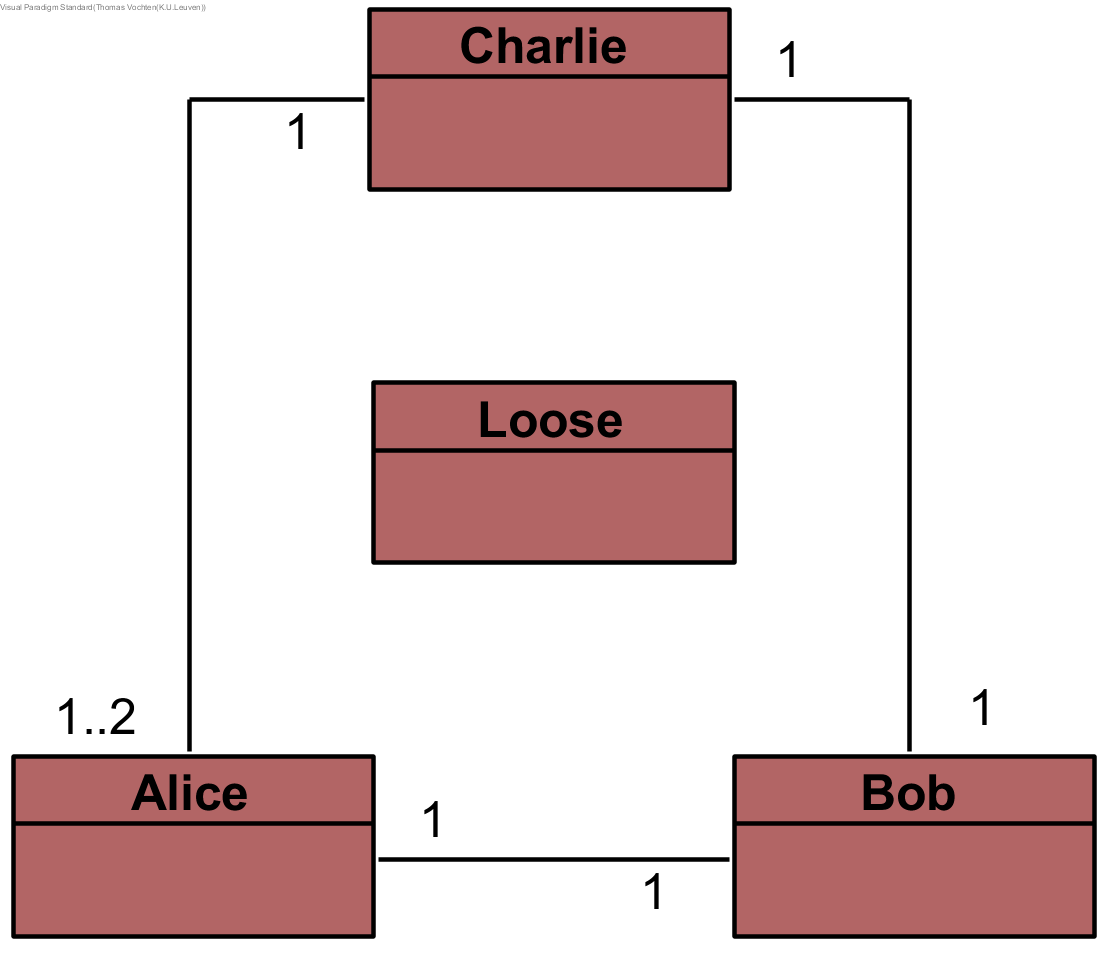
\includegraphics{chap-kwaliteitsgebrek/cycle.png}
	\caption{Voorbeeld van een onvoldoende precieze bovengrens in een klassehi\"erarchie en van een losstaande klasse (zijnde \textit{Loose})}
	\label{fig:cycle}
\end{figure}

\begin{figure}
	\centering
	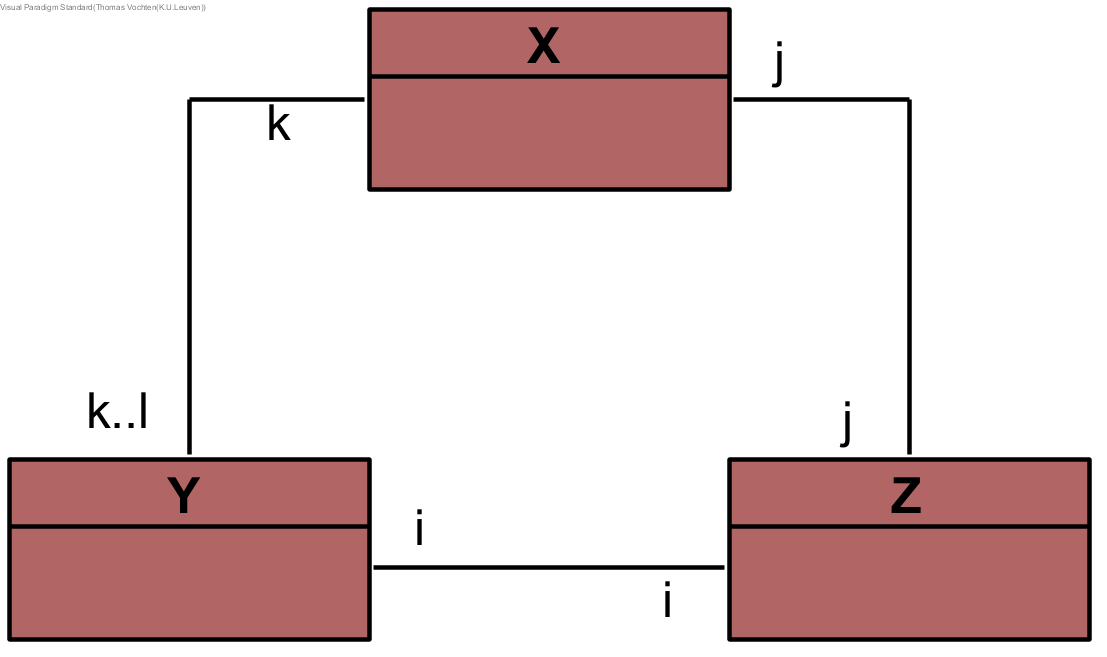
\includegraphics{chap-kwaliteitsgebrek/cyclegen.png}
	\caption{Het algemeen patroon voor onvoldoende precieze bovengrenzen}
	\label{fig:cyclegen}
\end{figure}

Zin \ref{form:manytomany} controleert of voor beide rollen van een associatie geldt dat de bovengrens * is.

Zin \ref{form:loose} controleert of klasse \textit{x} rechtstreeks geassocieerd is met een andere klasse, en zoniet, of klasse \textit{x} een subklasse is van een andere klasse en of die superklasse geassocieerd is met nog een andere klasse.

Zin \ref{form:imprecise-bound} controleert op patronen van associaties zoals in diagram \ref{fig:cyclegen}. De bovengrens op het uiteinde \textit{X} in een associatie \textit{X}---\textit{Y} wordt aangeduid als onvoldoende precies als er aan de volgende voorwaardes wordt voldaan:

\begin{itemize}
	\item \textit{X} en \textit{Y} moeten even veel instanties hebben.
	\item De ondergrens op het uiteinde \textit{X} is gelijk aan $k$ en de ondergrens en bovengrens op het uiteinde \textit{Y} zijn ook gelijk aan $k$.
	\item De bovengrens op het uiteinde \textit{X} is gelijk aan $l > k$ of $*$.
\end{itemize}

Bijlage \ref{app:kwaliteitsgebrek} bevat de theorie die werd gegenereerd uit een combinatie van diagrammen \ref{fig:diagram-voorbeeld} en \ref{fig:cycle}. IDP
vindt alle \textit{many-to-many} associaties en besluit dat \textit{Loose} een losstaande klasse is en verder dat de bovengrens op \textit{Alice} in de associatie \textit{Charlie}---\textit{Alice} onvoldoende precies is.